\documentclass{SeminarV2}
\usepackage{graphicx}
\usepackage[utf8]{inputenc}
\usepackage{amssymb,amsmath,array}
\usepackage[ngerman]{babel}
\usepackage{hyperref}

%***********************************************************************
% !!!! IMPORTANT NOTICE ON TEXT MARGINS !!!!!
%***********************************************************************
%
% Please avoid using DVI2PDF or PS2PDF converters: some undesired
% shifting/scaling may occur when using these programs
% It is strongly recommended to use the DVIPS converters.
%
% Check that you have set the paper size to A4 (and NOT to letter) in your
% dvi2ps converter, in Adobe Acrobat if you use it, and in any printer driver
% that you could use.  You also have to disable the 'scale to fit paper' option
% of your printer driver.
%
% In any case, please check carefully that the final size of the top and
% bottom margins is 5.2 cm and of the left and right margins is 4.4 cm.
% It is your responsibility to verify this important requirement.  If these margin requirements and not fulfilled at the end of your file generation process, please use the following commands to correct them.  Otherwise, please do not modify these commands.
%
\voffset 0 cm \hoffset 0 cm \addtolength{\textwidth}{0cm}
\addtolength{\textheight}{0cm}\addtolength{\leftmargin}{0cm}

%***********************************************************************
% !!!! USE OF THE SeminarV2 LaTeX STYLE FILE !!!!!
%***********************************************************************
%
% Some commands are inserted in the following .tex example file.  Therefore to
% set up your Seminar submission, please use this file and modify it to insert
% your text, rather than staring from a blank .tex file.  In this way, you will
% have the commands inserted in the right place.

% Edited by Martin Bogdan.

\begin{document}
%style file for Seminar manuscripts
\title{Row-Bot: Roboter essen Dreck auf}

%***********************************************************************
% AUTHORS INFORMATION AREA
%***********************************************************************
\author{Simon Hüning
%
% Optional short acknowledgment: remove next line if non-needed
%\thanks{This is an optional funding source acknowledgement.}
%
% DO NOT MODIFY THE FOLLOWING '\vspace' ARGUMENT
\vspace{.3cm}\\
%
% Addresses and institutions (remove "1- " in case of a single institution)
Universität Leipzig - Fakultät für Mathematik und Informatik \\
Augustusplatz 10, 04109 Leipzig - Deutschland
%
% Remove the next three lines in case of a single institution
%\vspace{.1cm}\\
%2- School of Second Author - Dept of Second Author \\
%Address of Second Author's school - Country of Second Author's school\\
}
%***********************************************************************
% END OF AUTHORS INFORMATION AREA
%***********************************************************************

\maketitle

\begin{abstract}
Rossiter et al. zeigen mit ihrem Row-Bot ein autonomes System mit der Fähigkeit, selbst Energie zu produzieren. Inspiriert von der Nahrungssuche und Fortbewegung der Ruderwanze wurde der Row-Bot für eine aquatische Umgebung entwickelt. Für die Energiegenerierung entnimmt eine mikrobielle Brennstoffzelle Biomasse aus ihrer Umgebung und treibt damit die Fortbewegung an, welche wiederum dafür sorgt, dass die Brennstoffzelle neue Biomasse aufnehmen kann. Dabei wird mehr Energie produziert als für die Nahrungsaufnahme benötigt wird. Die Arbeit könnte neue Wege für weitere Roboterentwicklungen mit eigenständiger Energieversorgung öffnen.
\end{abstract}

\section{Einführung}
Die Robotik steht vielen Herausforderungen gegenüber. Die Zeitdauer eines robotischen Systems autonom zu agieren zu verlängern, ist eine davon. Die meisten Roboter sind auf menschliche Hilfe angewiesen, um weiterhin funktionieren zu können. Es muss etwa die Batterie gewechselt oder der Treibstoff muss nachgefüllt werden, wenn dieser verbraucht ist. Dies ist in lebensbedrohlichen Umgebungen besonders schwierig. 

Bisherige Entwicklungen zeigen vielversprechende Ergebnisse, wie die Symbiotic Machine und der Eco-Bot. Diese Roboter nutzen eine Betankungstechnik analog zur Futtersuche biologischer Organismen. Die schwimmende Symbiotic Machine entnimmt Algen aus ihrer flüssigen Umgebung und erzeugt daraus Elektrolyte für die Redoxreaktion\footnote{"`Eine Redoxreaktion (eigentlich: Reduktions-Oxidations-Reaktion) ist eine chemische Reaktion, bei der ein Reaktionspartner Elektronen auf einen anderen überträgt."' \cite{redox}} in einer galvanischen Zelle. Aufgrund der Reaktion nimmt die Qualität der Zelle mit der Zeit ab. Der Eco-Bot nutzt im Gegensatz eine mikrobielle Brennstoffzelle (MBZ).  Der Eco-Bot besitzt mehrere gestapelte mikrobielle Brennstoffzellen, um Energie für Navigation und Bewegung zu gewinnen. Jedoch ist der Eco-Bot nur innerhalb der Reichweite der Futterstation operabel. Die gestapelten Brennstoffzellen erhöhen Größe und Komplexität des Roboters sowie Schwierigkeiten, die durch diese Technik verbunden sind.\cite[S. 3888]{DBLP:conf/iros/PhilamoreRSI15} Die MBZ beherbergt Mikroorganismen, die durch ihren Stoffwechsel Biomasse verarbeiten können. Die dadurch entstehende Redoxreaktion ermöglicht eine Energiegewinnung, die für spätere Aktionen gespeichert werden kann.\cite{MBZ} In vorangehenden Forschungen wurden Proben natürlicher Gewässertypen (Meer-, Süß-, Abwasser) als Quelle für Biomasse (Algen, Petrochemikalien) genutzt. Die möglichen Einsatzumgebung für auf Futtersuche befindliche Roboter ist daher vielseitig. Ebenso hat sich gezeigt, dass mikrobielle Brennstoffzellen auch in abgelegenen Umgebungen für eine längere Zeitdauer funktionsfähig bleiben. Die Ruderwanze (Abb. \ref{fig:ruderwanze}) bietet ein biologisches Vorbild für ein MBZ-betriebenes System mit autonomer Energieversorgung, den Row-Bot.\cite[S. 3888]{DBLP:conf/iros/PhilamoreRSI15}

\begin{figure}[ht]
\centering
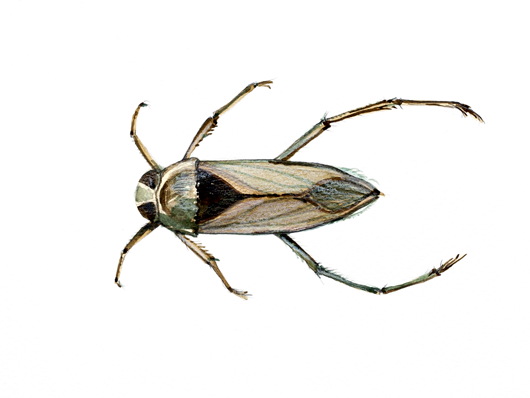
\includegraphics[width=0.3\textwidth]{pics/734-illustration-small}
\mycaption{Ruderwanze Quelle: \url{http://greensteps-assets.rec.org/organisms/insects/734-illustration-small.png} \label{fig:ruderwanze}}
\end{figure}

\section{Row-Bot}\label{sec:rowbot}

An den Row-Bot sind zwei Anforderungen gebunden.

\begin{enumerate}
\item Er muss selbstständig Energie gewinnen und speichern können.
\item Er muss sich bewegen und selbstständig neuen Treibstoff aufnehmen können. Der Vorgang darf nicht mehr Energie verbrauchen als vorher gewonnen wurde.
\end{enumerate}

Die erste Anforderung erfüllt die mikrobielle Brennstoffzelle. Die Höhe der generierten Energie ist davon abhängig, wie viel Biomaterial in der Arbeitsumgebung vorhanden ist. Die zweite Anforderung erfüllt ein Mechanismus, der dafür sorgt, dass durch die Bewegung neue Biomasse in die MBZ eingeführt wird. Um die Komplexität und Größe des \emph{Row-Bots} möglich gering zu halten, wird nur eine MBZ verwendet.\cite[S. 3889]{DBLP:conf/iros/PhilamoreRSI15}

\subsection{Aufbau}\label{sec:design}
\begin{figure}[ht]
\minipage{0.5\textwidth}
  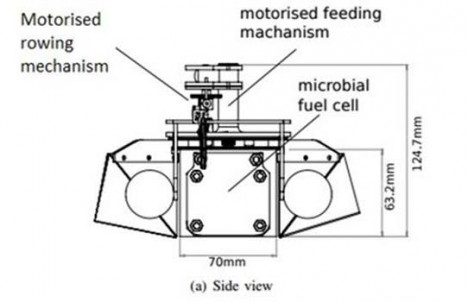
\includegraphics[width=\linewidth]{pics/front}
\endminipage\hfill
\minipage{0.5\textwidth}
  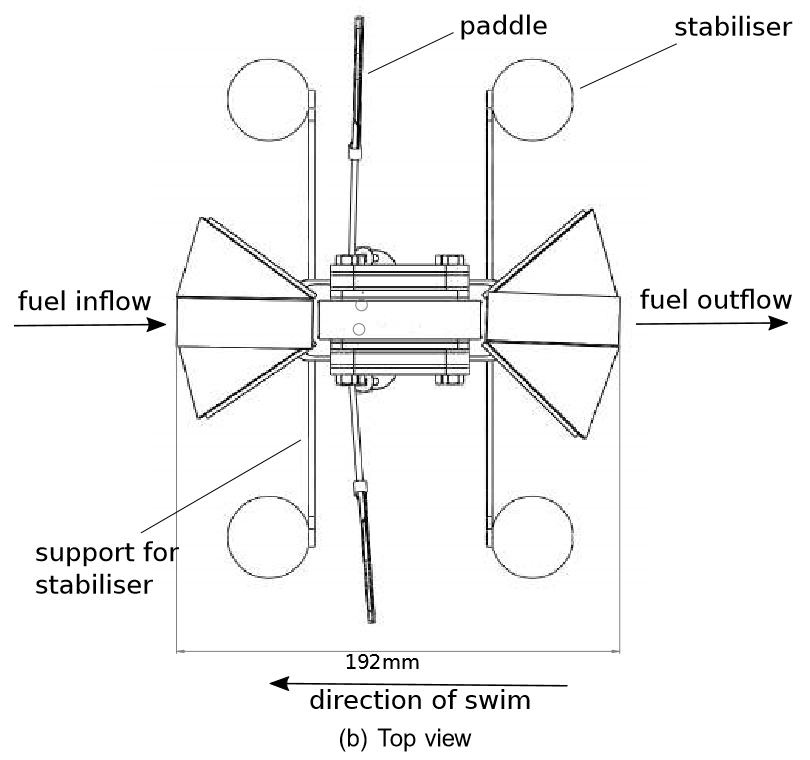
\includegraphics[width=0.7\linewidth]{pics/top}
\endminipage\hfill
\mycaption{CAD-Modell des Row-Bots mit geöffneten Durchlässen\cite{DBLP:conf/iros/PhilamoreRSI15}\label{fig:schema}}
\end{figure}
Das Design des Row-Bots wurde von der Ruderwanze abgeleitet. Die Ruderwanze findet sich hauptsächlich in kleinen Binnengewässern wie Teiche oder kleinere Seen mit einer hohen Dichte an Wasservegetation wie Algen. Algen gehören unter anderem zu der Nahrungsquelle der Ruderwanze. Sie zeigt auch eine effektive Fortbewegungsmethode, indem sie ihre mit Schwimmhaaren versehenen Hinterbeine als Ruder nutzt. Die Schwimmhaare sind so an den Beinen angebracht, dass sie während eines Schwimmzuges den Antrieb maximieren. Während sich die Beine nach einem Schwimmzug wieder in die Ausgangsposition bewegen, ziehen sich die Schwimmhaare zusammen, um einen Gegenantrieb zu minimieren.\cite[S. 3891]{DBLP:conf/iros/PhilamoreRSI15} Um an der Wasseroberfläche zu treiben, schließt sie Luft in eine Kammer innerhalb ihres Halsschildes ein. Das ermöglicht ihr auch die Atmung unter Wasser.\cite{ruderwanze} 

Die seitliche Ruderbewegung der Ruderwanze wurde ausgewählt, da diese im Vergleich zu anderen Käferarten mit Flachwasserhabitaten am besten mit der Form der MBZ verbinden lässt. Die MBZ ist zentral im Row-Bot platziert und übernimmt die Funktion des Verdauungstraktes. Seitlich an der MBZ sind jeweils mit einem Motor verbunden Paddel angebracht, die für die Vorwärtsbewegung sorgen. Damit neue Nahrung die MBZ passieren kann, sind vorne und hinten schließbare Öffnungen angebracht, welche auch jeweils durch einen Motor bewegt werden (Abb. \ref{fig:schema}). Ähnlich wie bei der Ruderwanze benutzt der Row-Bot auch Luftkammern, um an der Wasseroberfläche treiben zu können (Abb. \ref{fig:mbz}). Die Luftkammern geben auch Sauerstoff an die Kathode ab für die Redoxreaktion. Zur Stabilisierung der Konstruktion sind seitlich jeweils zwei Styroporkugeln angebracht.\cite[S. 3889 f.]{DBLP:conf/iros/PhilamoreRSI15}

\subsection{Energiegewinnung}\label{sec:energy}

\begin{figure}[ht]
\centering
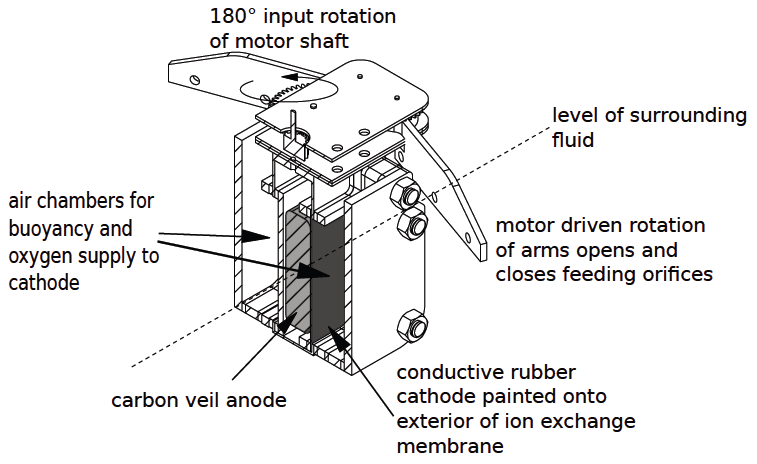
\includegraphics[width=0.5\textwidth]{pics/mfc}
\mycaption{CAD-Modell der MBZ\label{fig:mbz}}
\end{figure}

In eine mikrobielle Brennstoffzelle wurde mit Nährbrühe angereichertes Abwasser injiziert. Die Flüssigkeit in der Anodenkammer wurde täglich nach und nach mit einer Acetat-Stammlösung ausgetauscht. Nach fünf Tagen wurde der gesamte Inhalt der Anodenkammer erneut durch eine Acetat-Lösung mit einem anderen Pepton-Hefe-Beigemisch ausgetauscht.\cite[S. 3890]{DBLP:conf/iros/PhilamoreRSI15}

Nach dem Vorgang setzte man die MBZ in das Row-Bot-Gehäuse mit den motorisierten Öffnungen ein. Das Gehäuse wurde in ein kleines Wasserbecken gesetzt und an einer Angelschnur befestigt. Die Angelschnur war an einem motorisierten Zugmechanismus gekoppelt, welches das Gehäuse durch das Becken ziehen konnte. Das Becken wurde mit de-ionisiertem Wasser und einer geringen Menge Acetatlösung befüllt.\cite[S. 3890]{DBLP:conf/iros/PhilamoreRSI15}

In dem Becken öffnete man über manuelle Schalter die Futterdurchlässe über eine Dauer von 17 Sekunden. Nach drei Minuten zog man das Gehäuse entlang der Angelschnur $20cm$ mit einer durchschnittlichen Geschwindigkeit von $2,5cm/s$ durch das Becken. Dann wartete man eine Minute, bevor die Durchlässe wieder geschlossen wurden. Dies dauerte erneut 17 Sekunden.\cite[S. 3890]{DBLP:conf/iros/PhilamoreRSI15}

Da Energieoutput der MBZ gering ist (ungefähr $160mV$), wird dieser durch ein Spannungswandlermodul (EH4295  Micropower  Step  Up  Low  Voltage  Booster Module) auf $5,5V$ verstärkt. Durch die Effizienz des Spannungswandlers würde die MBZ über zehn Nahrungsaufnahmen hinweg $5J$ generieren. Die gewonnene Energie wurde in einem Kondensator gespeichert. Durch die Formel $E=CV^2/2$ lässt sich eine Kapazität von $330mF$ berechnen. Folgende Messungen haben gezeigt, dass der Spannungswandler eine Wandlungseffizienz von $30\%$ besitzt. So war der $330mF$ Kondensator mit $4,1V$ geladen. Unter Rücksicht der Wandlungseffizienz wurde eine neue Kapazität von $180mF$ berechnet, damit eine gewünschte Spannung von $5,5V$ erreicht wird.\cite[S. 3890]{DBLP:conf/iros/PhilamoreRSI15}

\subsection{Nahrungsaufnahme und Schwimmen}
\begin{figure}[ht]
\centering
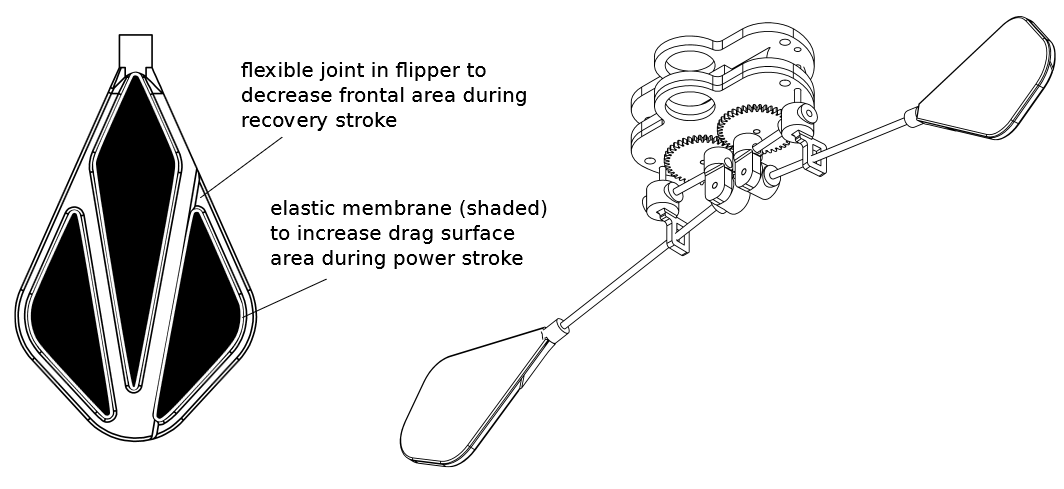
\includegraphics[width=0.7\textwidth]{pics/ruder}
\mycaption{CAD-Modell des Ruders\cite{DBLP:conf/iros/PhilamoreRSI15}\label{fig:ruder}}
\end{figure}

Um die Schwimmhaare der Ruderwanze (s. Kap.\ref{sec:design}) zu imitieren, sind die Ruder teilweise mit einer flexiblen Membran versehen. Diese vergrößert während eines Schwimmzuges ihre Oberfläche und sorgt so für einen größeren Vorderantrieb. Bei einem Schwimmzug befinden sich die Ruder unterhalb der Wasseroberfläche. Wenn die Ruder sich wieder in die Ausgangsposition zurückbewegen, werden die Paddel zu einem Großteil über Wasser gehoben, um einen Gegenantrieb zu minimieren. Die Fläche der Paddel, die sich noch unter Wasser befindet, ist mit einem Gelenk versehen. Das Gelenk klappt bei einem Rückführungszug ein und minimiert die Widerstand des Paddels. Das verkleinert ebenfalls einen Gegenantrieb.\cite[S. 3890 f.]{DBLP:conf/iros/PhilamoreRSI15}

Die Nahrungsaufnahmebewegungen (sequentiell: Durchlässe öffnen, Rudern, Durchlässe schließen) wurden ohne MBZ in einem Wasserbecken getestet. Die Gleichstrommotoren wurden nacheinander mit einem $330mF$ Kondensator mit einer Ladung von $4,1V$ und einem $180mF$ Kondensator mit einer Ladung von $5,5V$ betrieben (s. Kap. \ref{sec:energy}) und über manuelle Schalter angesteuert.\cite[S. 3891]{DBLP:conf/iros/PhilamoreRSI15}

\section{Ergebnisse}
\begin{figure}[ht]
\centering
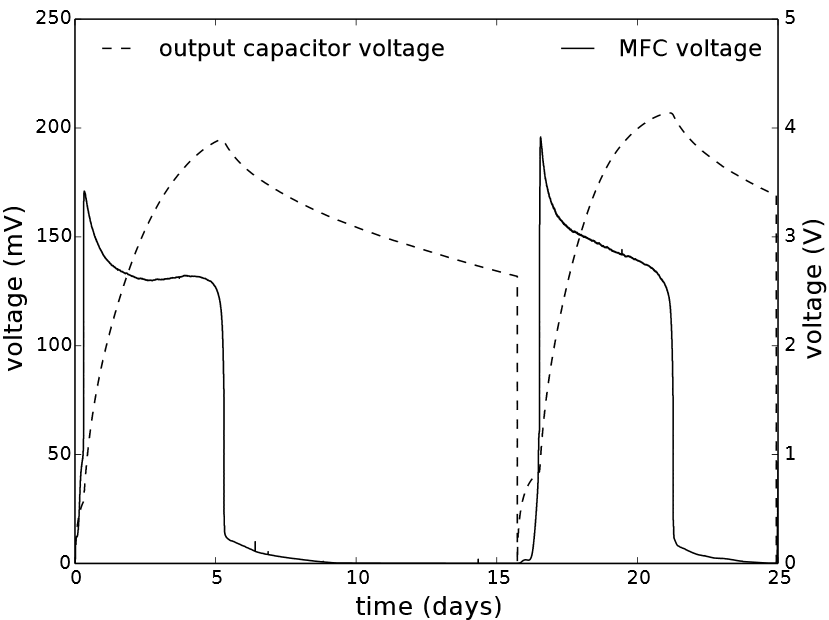
\includegraphics[width=0.4\textwidth]{pics/charge}
\mycaption{Ladungsverlauf des $330mF$ Kondensators\cite{DBLP:conf/iros/PhilamoreRSI15}\label{fig:charge}}
\end{figure}
Messungen der Ladung des $330mF$ Kondensators zeigten nach zwei aufeinanderfolgenden Fütterungen der MBZ eine Wandlungseffizienz von $30\%$. Der durchschnittliche Energieausstoß der MBZ betrug $8,82J$.

Die zwei Durchläufe über eine Ruderdistanz von $20cm$ mit dem $330mF$ und dem $180mF$ Kondensator wiesen folgende Messwerte auf:

\begin{figure}[ht]
\minipage{0.5\textwidth}
  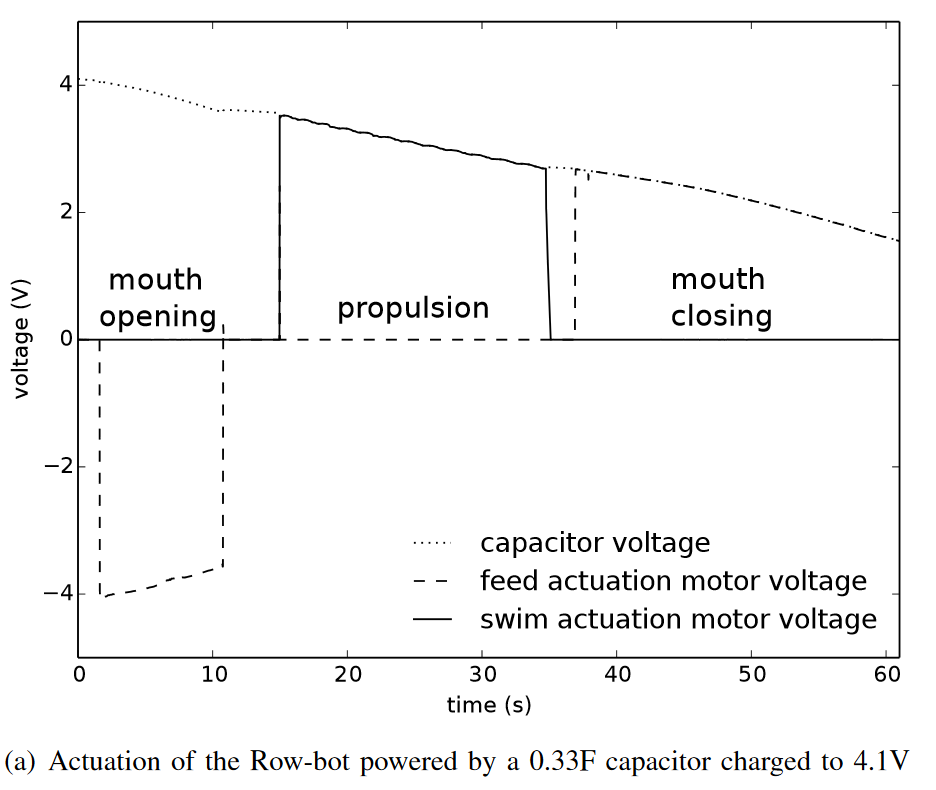
\includegraphics[width=0.7\linewidth]{pics/33}
\endminipage\hfill
\minipage{0.5\textwidth}
  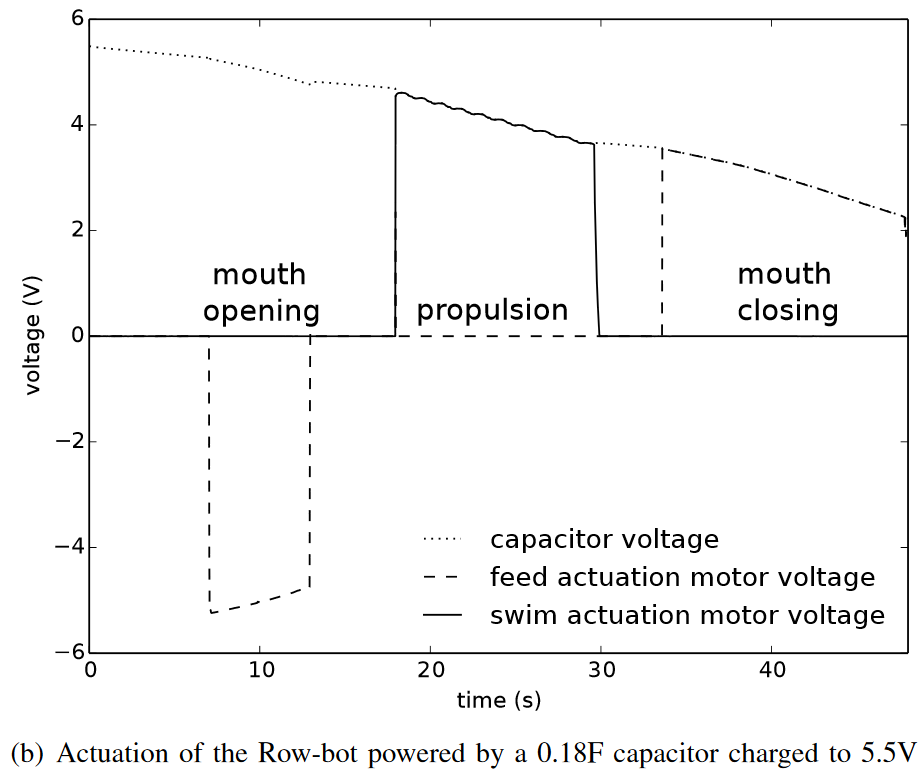
\includegraphics[width=0.7\linewidth]{pics/18}
\endminipage\hfill
\mycaption{Messdaten Nahrungsaufnahmebewegungen\cite{DBLP:conf/iros/PhilamoreRSI15}\label{fig:mess}}
\end{figure}

\begin{table}[h!]
  \centering
  \begin{tabular}{|c|c|c|c|c|c|c|c|c|c|}
    \hline
    Kapazität & Ladung & Öffnen & Rudern & Schließen &  Restenergie\\
    \hline
    $330mF$ & 4,$1V$ & $600mJ$ & $810mJ$ & $710mJ$ & $580mJ$ \\
    $180mF$ & 5,$5V$ & $410mJ$ & $700mJ$ & $690mJ$ & $900mJ$ \\
    \hline
  \end{tabular}
  \mycaption{Energiewerte Nahrungsaufnahmebewegungen\cite[S. 3892]{DBLP:conf/iros/PhilamoreRSI15}\label{tab:mess}}
\end{table}

Die Messwerte zeigen, dass nach dem Durchlauf der Bewegungen in beiden Fällen noch eine Restladung in den jeweiligen Kondensatoren verbleibt. Dabei stellt sich der $180mF$ Kondensator mit $900mJ$ Restenergie als am besten geeignet heraus. Jedoch lag die Schwimmleistung in beiden Fällen weit hinter der Ruderwanze zurück.\cite[S. 3891 f.]{DBLP:conf/iros/PhilamoreRSI15}

\section{Fazit und Ausblick}
Rossiter et al. zeigten mit ihrem Row-Bot Proof-of-Concept eine potentielle Möglichkeit für eine autonomische Energieversorgung nach dem Vorbild der Nahrungssuche der Ruderwanze. Der Row-Bot könnte in Schwärmen zukünftig für Einsätze als Umweltsensor oder Säuberung von Umweltverschmutzung konfiguriert werden.\cite{ted} Jedoch ist der Energieausstoß der MBZ mit synthetischen Futter höher ist, als mit rohem umweltschädlichem Nahrungsmaterial.\cite[S. 3892]{DBLP:conf/iros/PhilamoreRSI15} Spätere Entwicklungen des Row-Bots sollen ebenfalls die Antriebeffizienz steigern, indem der Körperaufbau der Ruderwanze weiter imitiert wird. Dazu gehört z.B. eine hydrophobe Haut.\cite[S. 3893]{DBLP:conf/iros/PhilamoreRSI15}

Im derzeitigen Stand der Entwicklung besteht der Row-Bot hauptsächlich aus Kunststoff. Würde es so zu einem Einsatz in abgelegenen Umgebungen kommen und dem Row-Bot ein Unfall widerfahren, wäre der Row-Bot selbst eine Quelle für Umweltverschmutzung. In einer späteren Präsentation stellte Rossiter den Plan vor, zukünftig biologisch abbaubare Materialien zu benutzen.\cite{ted}\cite{book:ross}

Die in Kap. {sec:rowbot} erwähnten Anforderungen wurden von Rossiters et al. Entwicklungen erfüllt und die verbleibende Restenergie kann für weitere Aktionen verwendet werden. Somit bietet der Row-Bot eine Grundlage für weiterführende Forschungen.

% ****************************************************************************
% BIBLIOGRAPHY AREA
% ****************************************************************************

\begin{footnotesize}

% ----------------------------------------------------------------------------

% IF YOU USE BIBTEX,
% - DELETE THE TEXT BETWEEN THE TWO ABOVE DASHED LINES
% - UNCOMMENT THE NEXT TWO LINES AND REPLACE 'Name_Of_Your_BibFile'

\bibliographystyle{unsrt}
\bibliography{main}

\end{footnotesize}

% ****************************************************************************
% END OF BIBLIOGRAPHY AREA
% ****************************************************************************

\end{document}
